\subsection{Model of college fund and education quality}
As is discussed above, the plan we made for the foundation lay special emphasis on the performance and competence of the graduates. As a result, we combined the graduation rate and the median salary after graduation to define a school's potential for effective use of private fundings.
To determine how we may invest on schools to optimize the utilization, it is necessary to first research the relationship between education and school funding. The following plot was plotted by scattering the average funding for each student($f_{avg}$) and the undergraduagte education quality($Q$). 
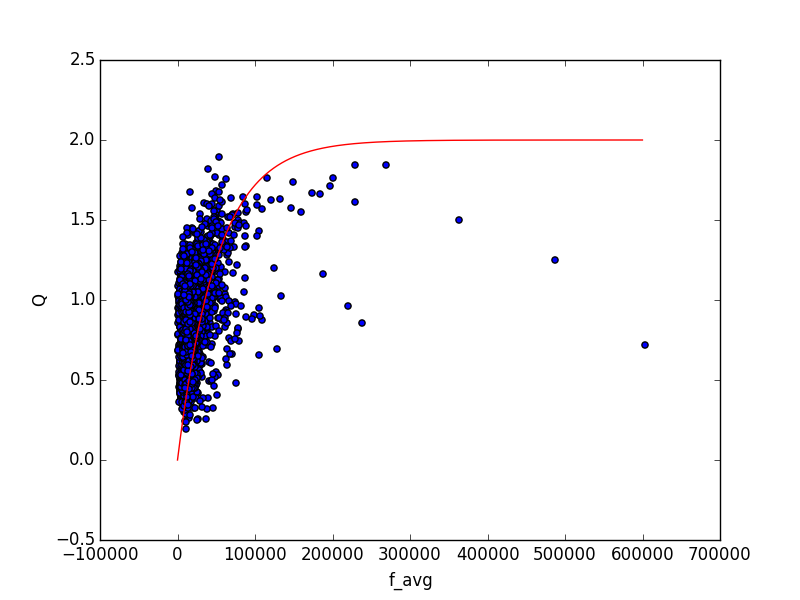
\includegraphics {f_q.png}

To fit a function $q(f_{avg})$ for the curve, following assumptions are made:
\begin{enumerate}
    \item If a school receives no fund at all, the education quality should be zero.
    \item Since the graduate rate and average salary are both mapped to $[0,1]$, $f(\inf)=2$ holds true for all possible functions
\end{enumerate}
A negative exponential function is used for fitting, that is 
$$q(f_{avg}) = b(1-e^{-Kf_{avg}}$$
$b=2$ and $K=1.96\times10^{-5}$ is used for the data set provided by the committee.
The descending trend of the gradient of the function indicates that investing on those compartively inferior collges may be a more preferred startegy, so in following work, the investment focuses on these schools.

\subsection{Clustering here}

\subsubsection{Model of the mutual influence among a cluster of schools}
It is widely recognized that the development a university may well influence all the universities in its neighbourhood. A feasible investment plan should take advantage of this fact so that it can improve the quality of the education in the whole region by only investing to a carefully selected subset of the local schools.

To model the mutual influence among clusters of schools, we made following assumptions:
\begin{enumerate}
    \item There is no mutual influence between schools belonging to different clusters.
    \item Among the same region, the influce of a school to another is inversely proportional to the distance between each other.
    \item The growth in a year will only influence the growth next year and the influce is proportional.
\end{enumerate}

Let $growth_{n} = [growth_{n}^{1}, growth_{n}^{2} \ldots , growth_{n}^{m}]$ be the growth vector of year n of the colleges in a region with m schools, then the mutual influence can be modeled as a mutal-influence matrix $G$ under the above assumptions:
$$growth_{n+1} = G growth_{n} $$
Where the elements $g_{ij}$ in $G$ is:
\begin{equation}
    g_{ij} =
    \begin{cases}
        1 &\mbox {if i=j}
        \lambda_{i}/distance_{ij} &\mbox {if i\neq j}
    \end{cases}
\end{equation}
The historical data of education quality in 2005, 2007, 2009, 2011 are used to fit the coefficients $\lambda_{i}$ for each college.
To validate the linear assumption, the correlation coefficient of the education quality of schools in the same region and different regions are calculated, most correlation coefficients of schools in the same region fall in the interval [0.8, 1.0], indicating that the performance of school in a same region are strongly positively correlated. On the other side, the correlation coefficients are relatively lower among different clusters. In our model, we simply assume that such correlation is caused by other factors and the performance of in one cluster has no influence on those in another. Thus the mutual-influence matrix $G$ for different regions 1 to k is $G = diag(G_{1}, G_{2} \ldot G{k})$.

\subsubsection{Model of the effect of investment in different regions}
Once the mutual-influence matrix $G$ is calculated, we can assess the effectiveness of investment in different regions. The model of the effect of funding on education quality is used to estimate the direct influence of the investment on each school:
The investment on each school 1 to n is $x=[x_{1}, x_{2} \ldots x_{n}]$. Thus the additional fund each student in each school is $\delta f_{avg}=[\delta f_{avg1}, \delta f_{avg2} \ldots \delta f_{avgn}]$, where $\delta f_{avgi} = x_{i} / student\_num_{i} (student\_num_{i}$ is the number of students in the ith college).
The direct improvement of education quality caused by investment is:
$$y = [y_{1}, y_{2} \ldots y_{n}] \mbox{where} y_{i} = q(f_{avgi} + \delta f_{avgi}) - q(f_avg{i})$$
After taking the mutual influence into account, the annual growth contributed by our investment is $Gy$. The solution to the following optimization problem makes best use of the funding from the foundation:
$$max Gy
s.t. \sum\limits_{i=1}^n student\_num_{i} \delta f_{avgi} = 100,000,000$$
We used an iterative manner to optimize the investment in five years. In each year the growth of education quality is turned into the equivalent growth of average funding $f_{avg}$ in each school and the optimization problem is solved again for the investment in the next year.
The clusters choosed from section ___ is used and the final optimiaztion result is such:


